% Percentage characters "%" that are meant to be printed need to be escaped like so: \%.

%% Copy and paste the code snippet below to add more content displayed conditionally (i.e., content to show if a particular value was selected for an option).
%% "OptionModelicaPath" should be replaced by the modelica path without dots of the option.
%% "Modelica.Path.Of.Selected.Value" should be replaced by the modelica path with dots of the selected value that should trigger the content to show in the document.
% \ifdefined\OptionModelicaPath
% \ifdefstring{\OptionModelicaPath}{Modelica.Path.Of.Selected.Value}{
% Text to display if the value returned by \OptionModelicaPath is equal to Modelica.Path.Of.Selected.Value.
% }{}
% \fi

\documentclass[10pt]{article}
\usepackage[letterpaper]{geometry} % Sets margins of the document based on US letter standard.
\usepackage{etoolbox} % Provides \ifdefstring command.
\usepackage{svg} % Provides \includesvg command. Please note that Inkscape must be in the path.
\usepackage{titlesec} % Provides \titleformat command.
\usepackage{enumitem}
\setlistdepth{5}

\setlist[itemize,1]{label=$\bullet$}
\setlist[itemize,2]{label=$\bullet$}
\setlist[itemize,3]{label=$\bullet$}
\setlist[itemize,4]{label=$\bullet$}
\setlist[itemize,5]{label=$\bullet$}
\renewlist{itemize}{itemize}{5}

\setlist[enumerate,1]{label=$\alph*.$}
\setlist[enumerate,2]{label=$\arabic*.$}
\setlist[enumerate,3]{label=$\roman*.$}
\setlist[enumerate,4]{label=$(\alph*)$}
\setlist[enumerate,5]{label=$(\arabic*)$}
\renewlist{enumerate}{enumerate}{5}

% Sets the path where SVGs are found.
% \svgpath{/Users/yves/Projects/lbnl/LBL-Linkage-Widget-v2/server/src/sequence/latex-assets/}

% If \basepath is not defined, use a fallback. Useful for editing the template outside of the backend.
\providecommand{\basepath}{/Users/yves/Projects/lbnl/LBL-Linkage-Widget-v2/server/src/sequence}

% Formats title
% https://en.wikibooks.org/wiki/LaTeX/Title_Creation
\title{Control Sequence}
\author{}
\date{}

% https://latex-programming.fandom.com/wiki/LaTeX_environment
\begin{document}

\maketitle

% Adds a page break.
% http://www.personal.ceu.hu/tex/breaking.htm
\newpage

% https://overleaf.com/learn/latex/Sections_and_chapters#Document_sectioning
% https://en.wikibooks.org/wiki/LaTeX/Labels_and_Cross-referencing
\section{Purpose}
\subsection{Information Provided by Designer}

\subsubsection{VAV Box Design Information}
\paragraph{VAV Cooling-Only Terminal Unit} \label{vav_cooling_only_terminal_unit}

\section{Scope}

\subsection{Generic Ventilation Zones} \label{generic_ventilation_zones}
\subsection{Generic Thermal Zones} \label{generic_thermal_zones}

\subsection{VAV Terminal Unit—Cooling Only}
\subsubsection{See “Generic Thermal Zones” (Section \ref{generic_thermal_zones}) for setpoints, loops, control modes, alarms, etc.}
\subsubsection{See “Generic Ventilation Zones” (Section \ref{generic_ventilation_zones}) for calculation of zone minimum outdoor airflow.}

CO2 DCV for cooling-only zones can lead to overcooling due to the faster rise in CO2 levels from people in the room versus the increase in cooling loads from people. Including heat in all zones with CO2 DCV is therefore recommended. 

\subsubsection{See Section \ref{vav_cooling_only_terminal_unit} for zone minimum airflow setpoint Vmin, zone maximum cooling airflow setpoint Vcool-max, and zone maximum heating airflow setpoint Vheat-max.}

If the minimum ventilation rate is more than 25\% or so of the cooling maximum, or DCV is used, a reheat box is recommended to avoid overcooling. DCV logic is not provided for cooling-only boxes, because doing so results in periods of overcooling, as the CO2 levels due to occupants rises much faster than the cooling load due to occupants because of thermal mass.

Cooling-only terminal units can provide heating only when the AHU supply air temperature is more than 3°C (5°F) above the room temperature.

\subsubsection{Active endpoints used in the control logic depicted in Figure \ref{figure:control_logic} shall vary depending on the mode of the Zone Group the zone is a part of (see Table \ref{figure:zone_group_mode}).}

\label{figure:zone_group_mode}
% Inserts a table.
\begin{center}
Table \ref{figure:zone_group_mode} Endpoints as a Function of Zone Group Mode 
\end{center}
%
% https://es.overleaf.com/learn/latex/Tables
\begin{tabular}{ c|c|c|c|c|c|c } 
 \hline
 Endpoint & Occupied & Cooldown & Setup & Warmup & Setback & Unoccupied \\ 
 \hline
 Cooling maximum & Vcool-max & Vcool-max & Vcool-max & 0 & 0 & 0 \\ 
 \hline
 Minimum & Vmin* & 0 & 0 & 0 & 0 & 0 \\ 
 \hline
 Heating maximum & Vheat-max & 0 & 0 & Vcool-max & Vcool-max & 0 \\ 
 \hline
\end{tabular}

\subsubsection{Control logic is depicted schematically in Figure \ref{figure:control_logic} and described in the following subsections.} \label{figure:control_logic}

% Inserts PDF image
\begin{figure}[h]
  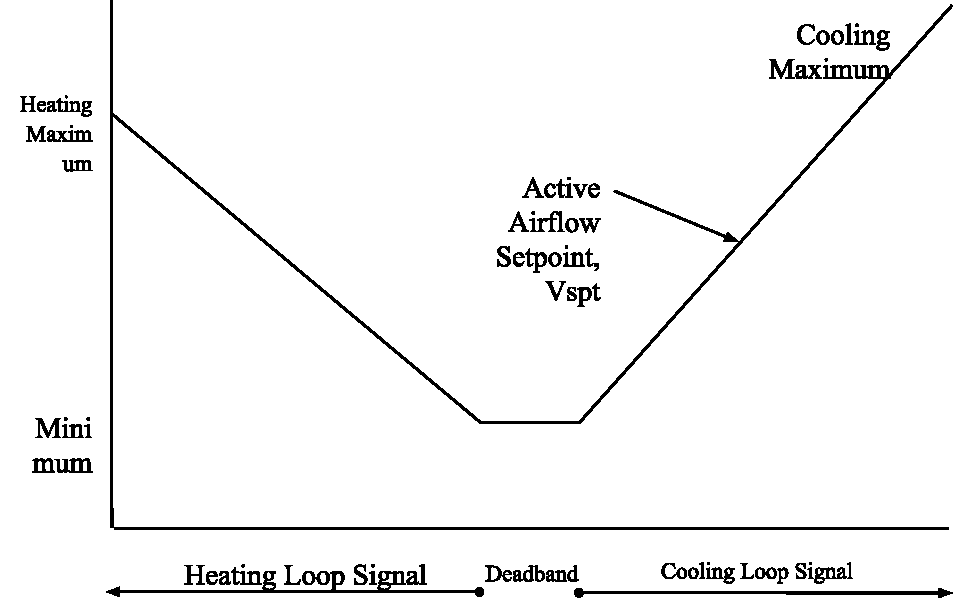
\includegraphics{\basepath/converted-latex-assets/control-logic_svg-tex.pdf}
\end{figure}

% Inserts PNG
\begin{figure}[h]
  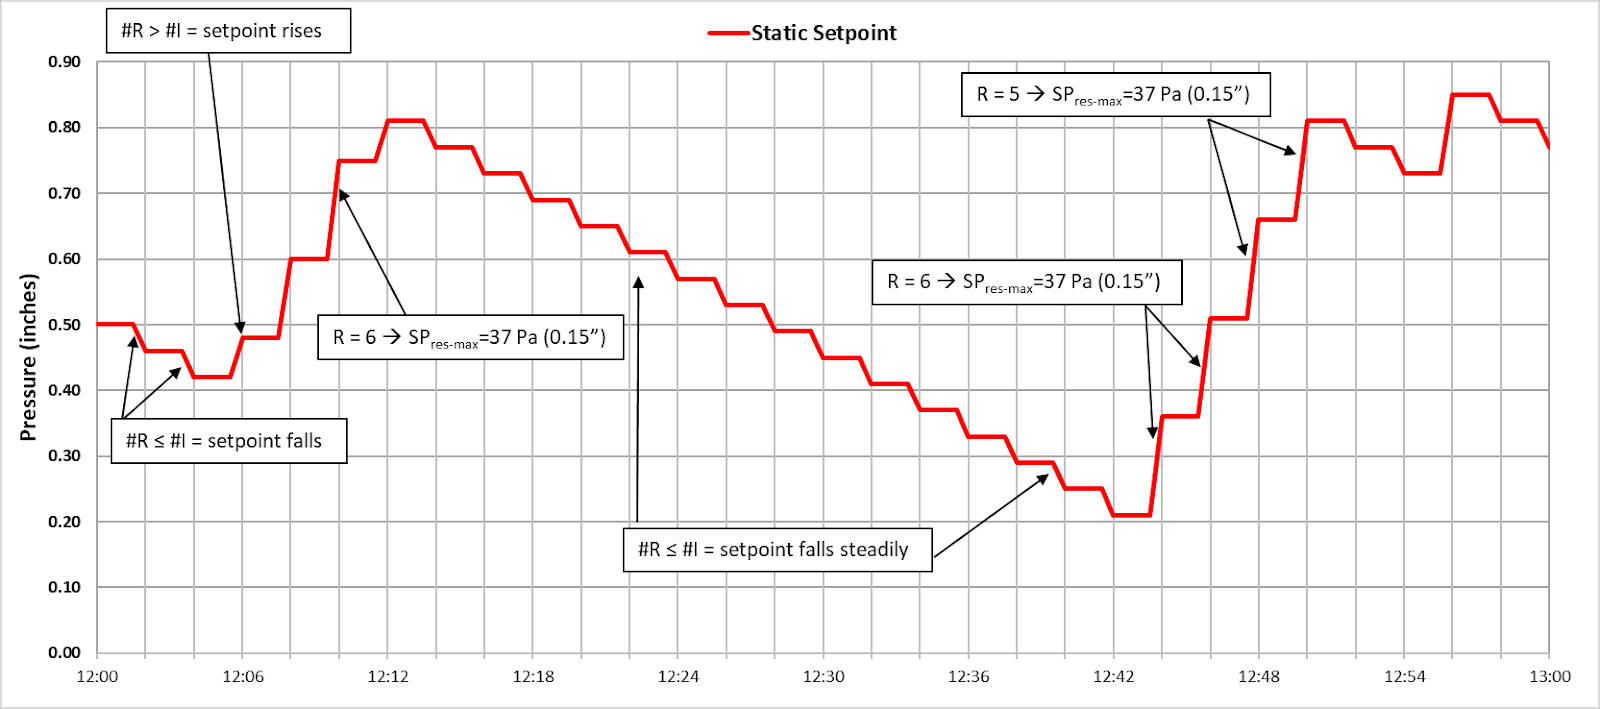
\includegraphics{\basepath/latex-assets/image6.png}
\end{figure}

\ifdefined\BuildingsTemplatesAirHandlersFansInterfacesPartialAirHandlertypFanRet
\ifdefstring{\BuildingsTemplatesAirHandlersFansInterfacesPartialAirHandlertypFanRet}{Buildings.Templates.Components.Types.Fan.SingleConstant}{
Type of return fan: Single fan - Constant speed
}{}
\fi

\section{Setpoints, Design and Field Determined}
\section{List of Hardwired Points}
\section{Sequences of Operations}

\subsection{General}

\subsection{Generic Ventilation Zones}

\textit{A ventilation zone is a space or group of spaces served by one ventilation control device. For VAV systems, ventilation zones and thermal zones are one and the same, but Guideline 36 will eventually be expanded to include dedicated outdoor air systems (DOAS) serving one or more thermal zones controlled by radiant systems, chilled beams, fan-coils, etc.}

Zone Minimum Outdoor Air and Minimum Airflow Setpoints

\paragraph{For every zone that requires mechanical ventilation, the zone minimum outdoor airflows and setpoints shall be calculated depending on the governing standard or code for outdoor air requirements.}

\paragraph{See Section 3.1.2 for zone minimum airflow setpoint Vmin.}

\ifdefined\ASHRAEStandard
  \paragraph{For compliance with the Ventilation Rate Procedure of ASHRAE Standard 62.1-2016, outdoor air and zone minimum setpoints shall be calculated as follows:}
  \begin{enumerate}
    \item See Section 3.1.1.2 for zone ventilation setpoints.
    \item Determine zone air distribution effectiveness Ez.
    \begin{enumerate}
      \item If the DAT at the terminal unit is less than or equal to zone space temperature, Ez shall be equal to EzC (default to 1.0 if no value is scheduled).
      \item If the DAT at the terminal unit is greater than zone space temperature, Ez shall be equal to EzH (default to 0.8 if no value is scheduled).
    \end{enumerate}
    \item Vbz-P* is the population component of the required breathing zone outdoor airflow. The normal value of Vbz-P* shall be Vbz-P. Vbz-A* is the area component of the required breathing zone outdoor airflow.  The normal value of Vbz-A* shall be Vbz-A.
    \item Vmin
    \begin{enumerate}
      \item Shall be equal to Voz as calculated in Section 5.2.1.3.f below if Vmin in Section 3.1.2 is “AUTO” and the associated air handler has been supplying 100\% outdoor air (outdoor air damper fully open; return air damper fully closed) for 10 minutes;
      \item Else shall be equal to 1.5 * Voz as calculated in Section 5.2.1.3.f below if Vmin in Section 3.1.2 is “AUTO” and the associated air handler is not supplying 100\% outdoor air;
      \item Else shall be equal Vmin as entered in Section 3.1.2.
    \end{enumerate}
    \item The occupied minimum airflow Vmin* shall be equal to Vmin except as noted in Section 5.2.1.3.f.
    \item The required zone outdoor airflow Voz shall be calculated as Voz = (Vbz-A* + Vbz-P*)/Ez, where the normal values of Vbz-A* and Vbz-P* are modified if any of the following conditions are met, in order from higher to lower priority:
    \begin{enumerate}
      \item If the zone is in any mode other than Occupied Mode, and for zones that have window switches and the window is open: Vbz-P* = 0, Vbz-A* = 0, and Vmin* = 0.
      \item If the zone has an occupancy sensor, is unpopulated, and occupied-standby mode is permitted: Vbz-P* = 0, Vbz-A* = 0, and Vmin* = 0.
      \item Else, if the zone has an occupancy sensor, is unpopulated, but occupied-standby mode is not permitted: Vbz-P* = 0 and Vmin* = Vmin.
      \textit{Occupied-standby mode applies to individual zones, is considered a zonal subset of Occupied Mode, and is not considered a zone-group operating mode.}
      \item If the zone has a CO2 sensor:
      \begin{enumerate}
        \item See Section 3.1.1.2.b.3 for CO2 setpoints.
        \item During Occupied Mode, a P-only loop shall maintain CO2 concentration at setpoint; reset from 0\% at setpoint minus 200 PPM and to 100\% at setpoint. 
        \item Loop is disabled and output set to zero when the zone is not in Occupied Mode.
        \textit{CO2 DCV is not yet well defined for Standard 62.1. RP-1747 is under way and should provide a detailed procedure. In the meantime, sequences have been included at the zone level, matching California’s DCV approach as a first step. Because outdoor air rates at the AHU level dynamically calculate outdoor air rates using the Standard 62.1 multiple-spaces procedure, compliance with the standard is assured. Doing no DCV at all is not an option, because it is required by Standard 90.1-2016.}
        \item For cooling-only VAV terminal units, reheat VAV terminal units, constant-volume series fan-powered terminal units, dual-duct VAV terminal units with mixing control and inlet airflow sensors, dual-duct VAV terminal units with mixing control and a discharge airflow sensor, or dual-duct VAV terminal units with cold-duct minimum control:
        \begin{enumerate}
          \item The CO2 control loop output shall reset both the occupied minimum airflow setpoint (Vmin*) and the population component of the required breathing zone outdoor airflow (Vbz-P*) in parallel. Vmin* shall be reset from the zone minimum airflow setpoint Vmin at 0\% loop output up to maximum cooling airflow setpoint Vcool-max at 100\% loop output. Vbz-P* shall be reset from 0 L/s (0 cfm) at 0\% loop output up to the Vbz-P at 100\% loop output. See Figure 5.2.1.3-1.
          \textit{The CO2 control loop graph in Figure 5.2.1.3-1 is provided as a visual representation of the reset logic and is not representative of magnitude of Vbz-P* in relation to Vbz-A or Vmin*.}
        \end{enumerate}
        \item For parallel fan-powered terminal units:
        \begin{enumerate}
          \item Determine VCO2-max as follows:
          \begin{enumerate}
           \item When the Zone State is cooling, VCO2-max is equal to the maximum cooling airflow setpoint Vcool-max.
           \item When the Zone State is heating or deadband, VCO2-max is equal to Vcool-max minus the parallel fan airflow
           \textit{This logic prevents the total supply airflow from exceeding Vcool-max, which could create diffuser noise problems.}
          \end{enumerate}
          \item The CO2 control loop output shall reset both the occupied minimum airflow setpoint Vmin* and the population component of the required breathing zone outdoor airflow Vbz-P* in parallel. Vmin* shall be reset from the zone minimum airflow setpoint Vmin at 0\% loop output up to maximum cooling airflow setpoint VCO2-max at 100\% loop output. Vbz-P* shall be reset from 0 L/s (0 cfm) at 0\% loop output up to the Vbz-P at 100\% loop output. See Figure 5.2.1.3-2.
          \textit{The CO2 control loop graph in Figure 5.1.2.1.3-2 is provided as a visual representation of the reset logic and is not representative of magnitude of Vbz-P* in relation to Vbz-A or Vmin*.}
          \item For SZVAV AHUs:
          \begin{enumerate}
            \item The minimum outdoor air setpoint MinOAsp is equal to Voz. The CO2 control loop output shall reset the population component of the required breathing zone outdoor airflow Vbz-P* from 0 L/s (0 cfm) at 0\% loop output up to Vbz-P at 100\% loop output. See Figure 5.2.1.3-3.    
          \end{enumerate}
        \end{enumerate}
      \end{enumerate}
    \end{enumerate}
  \end{enumerate}
\fi
\ifdefined\CaliforniaTitle
  \paragraph{For compliance with California Title 24, outdoor air setpoints shall be calculated as follows:}
  \begin{enumerate}
    \item See Section 3.1.1.2 for zone ventilation setpoints.
    \item Determine the zone minimum outdoor air setpoints Zone-Abs-OA-min and Zone-Des-OA-min.
    \textit{Zone-Abs-OA-min is used in terminal-unit sequences and air-handler sequences. Zone-Des-OA-min is used in air-handler sequences only.}
    \begin{enumerate}
      \item Zone-Abs-OA-min shall be reset based on the following conditions in order from highest to lowest priority:
      \begin{enumerate}
        \item Zero if the zone has a window switch and the window is open.
        \item Zero if the zone has an occupancy sensor and is unpopulated and is permitted to be in occupied-standby mode per Section 3.1.1.2.b.3.
        \textit{The term “populated” is used instead of “occupied” to mean that a zone occupancy sensor senses the presence of people, because the term “occupied” is used elsewhere to mean “scheduled to be occupied.”}
        \item Varea-min if the zone has a CO2 sensor.
        \item Zone-Des-OA-min otherwise.
      \end{enumerate}
      \item Zone-Des-OA-min is equal to the following, in order from highest to lowest priority:
      \begin{enumerate}
        \item Zero if the zone has a window switch and the window is open.
        \item Zero if the zone has an occupancy sensor, is unpopulated, and is permitted to be in occupied-standby mode per Section 3.1.1.2.b.3.
        \item The larger of Varea-min and Vocc-min otherwise.
      \end{enumerate}
    \end{enumerate}
    \item Vmin
    \begin{enumerate}
      \item Shall be equal to Zone-Abs-OA-min if Vmin in Section 3.1.2 is “AUTO”;
      \item Else shall be equal to Vmin as entered in Section 3.1.2.
    \end{enumerate}
    \item The occupied minimum airflow Vmin* shall be equal to Vmin except as noted below, in order from highest to lowest priority:
    \begin{enumerate}
      \item If the zone has an occupancy sensor and is permitted to be in occupied-standby mode per Section 3.1.1.2.b.3, Vmin* shall be equal to zero when the room is unpopulated.
      \item If the zone has a window switch, Vmin* shall be zero when the window is open.
      \item If the zone has a CO2 sensor:
      \begin{enumerate}
        \item See Section 3.1.1.2.b.3 for CO2 setpoints.
        \item During Occupied Mode, a P-only loop shall maintain CO2 concentration at setpoint; reset from 0\% at setpoint minus 200 PPM and to 100\% at setpoint. 
        \item Loop is disabled and output set to zero when the zone is not in Occupied Mode.
        \item For cooling-only VAV terminal units, reheat VAV terminal units, constant-volume series fan-powered terminal units, dual-duct VAV terminal units with mixing control and inlet airflow sensors, dual-duct VAV terminal units with mixing control and a discharge airflow sensor, or dual-duct VAV terminal units with cold-duct minimum control:
        \begin{enumerate}
          \item The CO2 control loop output shall reset the occupied minimum airflow setpoint Vmin* from the zone minimum airflow setpoint Vmin at 0\% up to maximum cooling airflow setpoint Vcool-max at 50\%, as shown in Figure 5.2.1.4-1. The loop output from 50\% to 100\% will be used at the system level to reset outdoor air minimum; see AHU controls.
        \end{enumerate}
        \item For parallel fan-powered terminal units:
        \begin{enumerate}
          \item Determine VCO2-max as follows:
          \begin{enumerate}
            \item When the Zone State is cooling, VCO2-max is equal to the maximum cooling airflow setpoint Vcool-max.
            \item When the Zone State is heating or deadband, VCO2-max is equal to Vcool-max minus the parallel fan airflow
          \end{enumerate}
          \textit{This logic prevents the total supply airflow from exceeding Vcool-max, which could create diffuser noise problems.}
          \item The CO2 control loop output shall reset the occupied minimum airflow setpoint Vmin* from the zone minimum airflow setpoint Vmin at \% up to maximum cooling airflow setpoint VCO2-max at 50\%, as shown in Figure 5.2.1.4-2. The loop output from 50\% to 100\% will be used at the system level to reset outdoor air minimum; see AHU controls.
        \end{enumerate}
        \item For SZVAV AHUs:
        \begin{enumerate}
         \item The minimum outdoor air setpoint MinOAsp shall be reset based on the zone CO2 control-loop signal from MinOA at 0\% signal to DesOA at 100\% signal. See Figure 5.2.1.4-3.
        \end{enumerate}
      \end{enumerate}
    \end{enumerate}
    \item When Zone State is Deadband
    \begin{enumerate}
      \item FANsp shall be DeadbandSpeed.  If DeadbandSpeed is zero, shut the fan off.
      \item Cooling coil \textsc{off}
      \item Heating coil \textsc{off}
    \end{enumerate}
    \item If there is a cooling coil, when Zone State is Cooling
    \begin{enumerate}
      \item For a cooling-loop signal of 0\% to 50\%, FANsp is MinCoolSpeed.
      \item For a cooling-loop signal of 50\% to 100\%, FANsp is reset from MinCoolSpeed to MaxCoolSpeed.
      \item For a cooling-loop signal of 0\% to 50\%, SATsp is reset from the active zone cooling setpoint to Cool\_SAT.
      \item For a cooling-loop signal of 50\% to 100\%, SATsp is Cool\_SAT.   
      \item The cooling coil shall be modulated with a PID loop to maintain the discharge temperature at SATsp.
      \item Heating coil \textsc{off}
    \end{enumerate}
  \end{enumerate}
\fi

\end{document}
